
\begin{figure*}[t]
    \centering
    % --- Row 1 ---
    \subfloat[SW ($n=4$)]{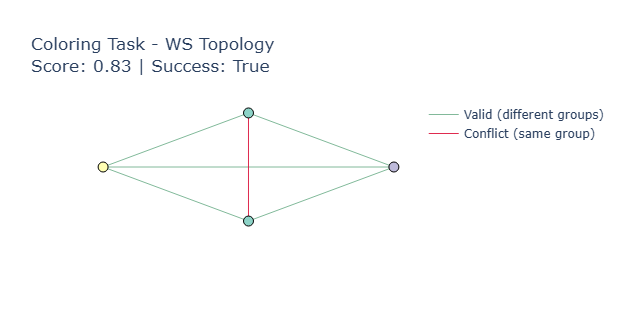
\includegraphics[trim=90 80 200 100,clip,width=0.12\textwidth]{figures/topology/coloring_results_20250917_222432_rounds8_gpt-4o-mini_nodes4.png}}
    \subfloat[SW ($n=8$)]{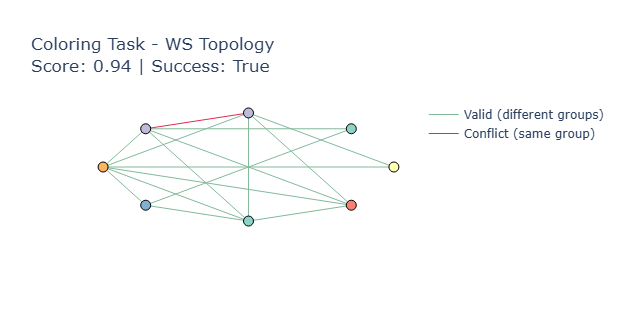
\includegraphics[trim=90 80 200 100,clip,width=0.16\textwidth]{figures/topology/coloring_results_20250917_222635_rounds8_gpt-4o-mini_nodes8.png}}
    \subfloat[SW ($n=16$)]{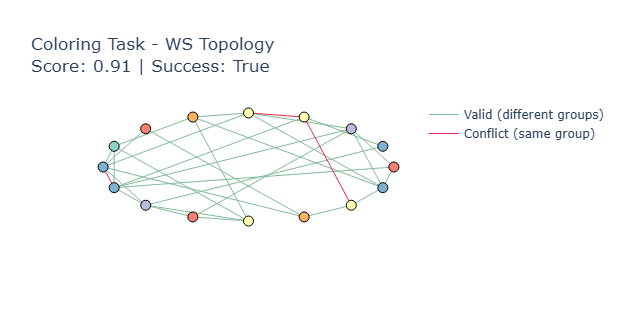
\includegraphics[trim=90 80 200 100,clip,width=0.19\textwidth]{figures/topology/coloring_results_20250917_222842_rounds8_gpt-4o-mini_nodes16.png}}
    \subfloat[SW ($n=50$)]{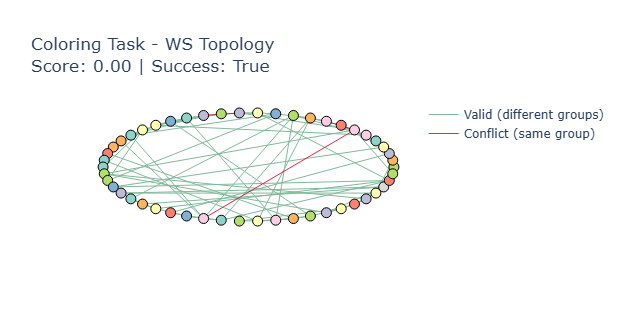
\includegraphics[trim=90 80 200 100,clip,width=0.22\textwidth]{figures/topology/coloring_results_20250920_135347_rounds11_gpt-4o-mini_nodes50.png}}
    \subfloat[SW ($n=100$)]{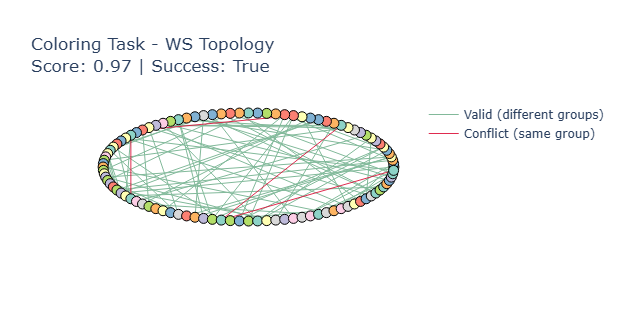
\includegraphics[trim=90 80 200 100,clip,width=0.26\textwidth]{figures/topology/coloring_results_20250920_141018_rounds15_gpt-4o-mini_nodes100.png}}

    % --- Row 2 ---
    \subfloat[SF ($n=4$)]{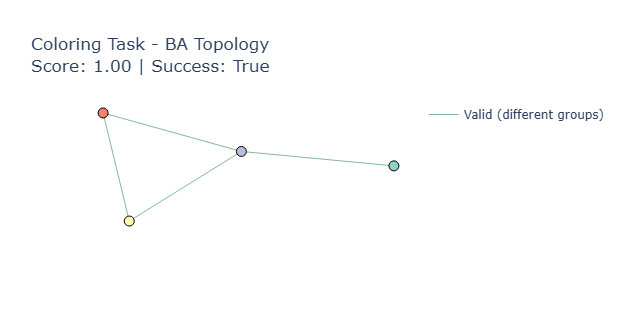
\includegraphics[trim=90 80 200 100,clip,width=0.12\textwidth]{figures/topology/coloring_results_20250917_223003_rounds8_gpt-4o-mini_nodes4.png}}
    \subfloat[SF ($n=8$)]{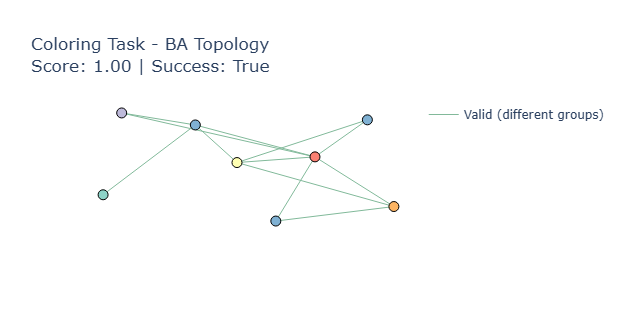
\includegraphics[trim=90 80 200 100,clip,width=0.16\textwidth]{figures/topology/coloring_results_20250917_223205_rounds8_gpt-4o-mini_nodes8.png}} 
    \subfloat[SF ($n=16$)]{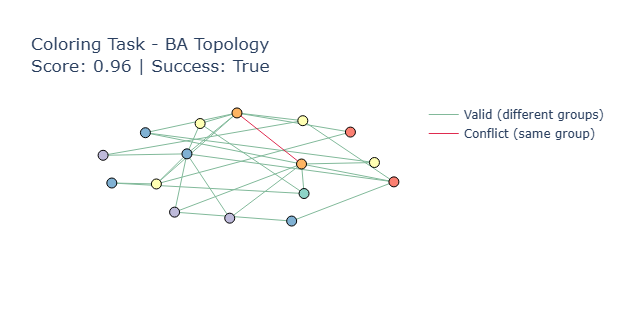
\includegraphics[trim=90 80 200 100,clip,width=0.19\textwidth]{figures/topology/coloring_results_20250917_223421_rounds8_gpt-4o-mini_nodes16.png}}
    \subfloat[SF ($n=50$)]{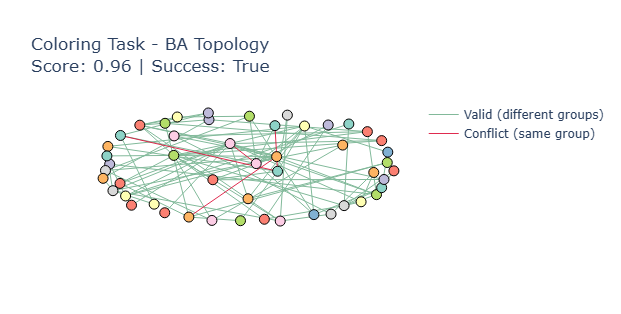
\includegraphics[trim=90 80 200 100,clip,width=0.22\textwidth]{figures/topology/coloring_results_20250920_141717_rounds11_gpt-4o-mini_nodes50.png}}
    \subfloat[SF ($n=100$)]{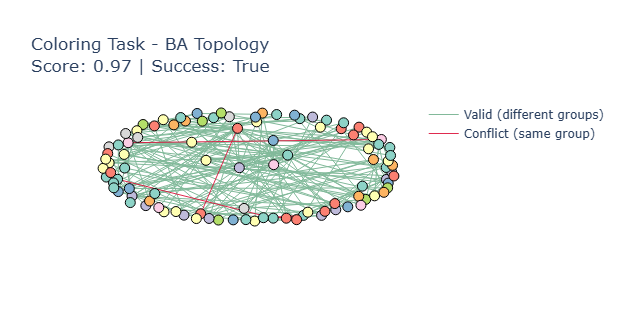
\includegraphics[trim=90 80 200 100,clip,width=0.26\textwidth]{figures/topology/coloring_results_20250920_142903_rounds11_gpt-4o-mini_nodes100.png}}

    % --- Row 3 ---
    \subfloat[DT ($n=4$)]{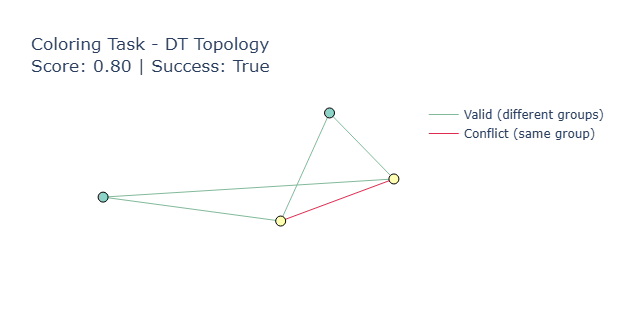
\includegraphics[trim=90 80 200 100,clip,width=0.12\textwidth]{figures/topology/coloring_results_20250917_223636_rounds8_gpt-4o-mini_nodes4.png}}
    \subfloat[DT ($n=8$)]{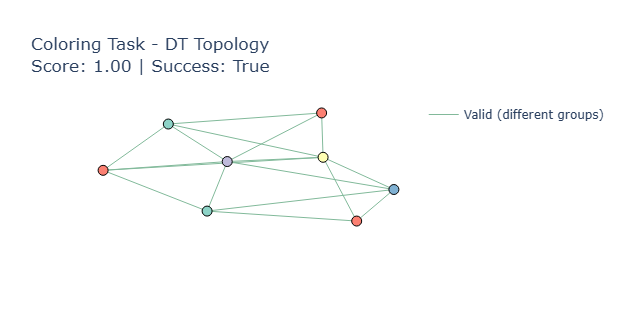
\includegraphics[trim=90 80 200 100,clip,width=0.16\textwidth]{figures/topology/coloring_results_20250917_223854_rounds8_gpt-4o-mini_nodes8.png}}
    \subfloat[DT ($n=16$)]{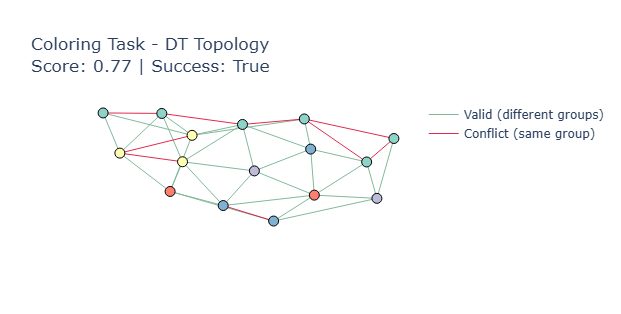
\includegraphics[trim=90 80 200 100,clip,width=0.19\textwidth]{figures/topology/coloring_results_20250917_224151_rounds8_gpt-4o-mini_nodes16.png}} 
    \subfloat[DT ($n=50$)]{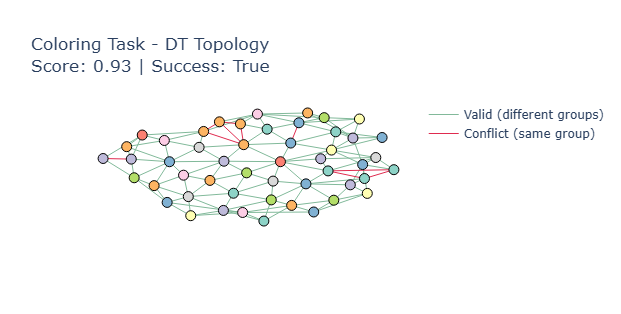
\includegraphics[trim=90 80 200 100,clip,width=0.22\textwidth]{figures/topology/coloring_results_20250920_143802_rounds13_gpt-4o-mini_nodes50.png}} 
    \subfloat[DT ($n=100$)]{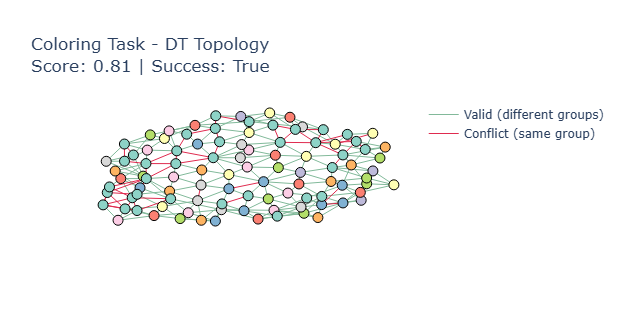
\includegraphics[trim=90 80 200 100,clip,width=0.26\textwidth]{figures/topology/coloring_results_20250920_145919_rounds19_gpt-4o-mini_nodes100.png}} \\



    \vspace{2mm}
    % --- Row 4 ---
    \subfloat[Seq. ($n=4$)]{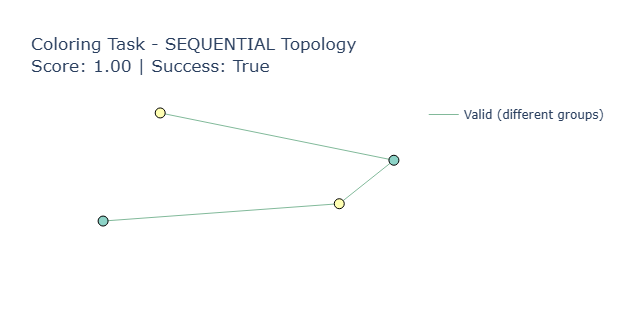
\includegraphics[trim=90 80 200 100,clip,width=0.12\textwidth]{figures/topology/coloring_results_20250924_130551_rounds8_gpt-4o-mini_nodes4.png}}
    \subfloat[Seq. ($n=8$)]{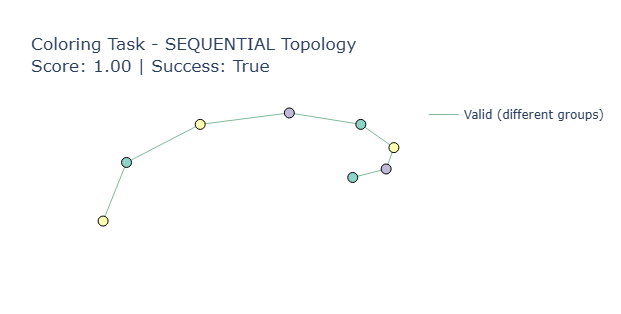
\includegraphics[trim=90 80 200 100,clip,width=0.16\textwidth]{figures/topology/coloring_results_20250924_130747_rounds8_gpt-4o-mini_nodes8.png}}
    \subfloat[Seq. ($n=16$)]{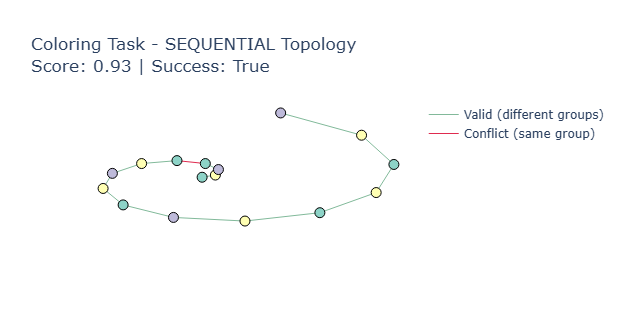
\includegraphics[trim=90 80 200 100,clip,width=0.19\textwidth]{figures/topology/coloring_results_20250924_131004_rounds8_gpt-4o-mini_nodes16.png}} 
    \subfloat{\rule{0.22\textwidth}{0pt}} % placeholder without number
    \subfloat{\rule{0.26\textwidth}{0pt}} % placeholder without number



    % --- Row 5 ---
    \subfloat[Hier. ($n=4$)]{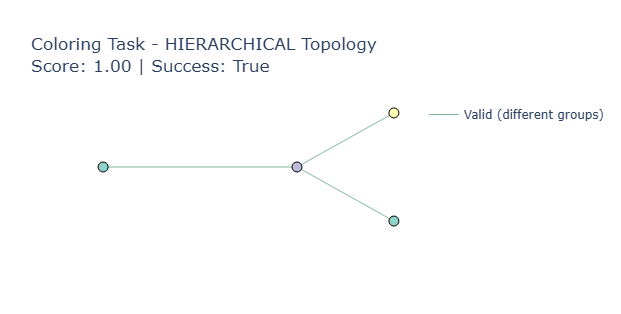
\includegraphics[trim=90 80 200 100,clip,width=0.12\textwidth]{figures/topology/coloring_results_20250924_143605_rounds8_gpt-4o-mini_nodes4.png}}
    \subfloat[Hier. ($n=8$)]{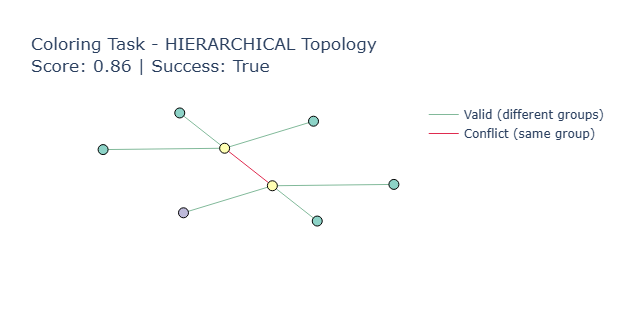
\includegraphics[trim=90 80 200 100,clip,width=0.16\textwidth]{figures/topology/coloring_results_20250924_143802_rounds8_gpt-4o-mini_nodes8.png}}
    \subfloat[Hier. ($n=16$)]{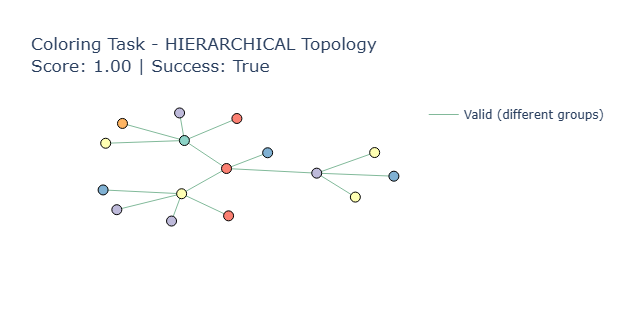
\includegraphics[trim=90 80 200 100,clip,width=0.19\textwidth]{figures/topology/coloring_results_20250924_144052_rounds8_gpt-4o-mini_nodes16.png}} 
    \subfloat[Hier. ($n=50$)]{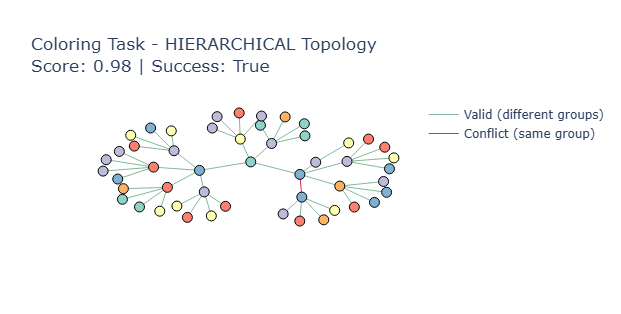
\includegraphics[trim=90 80 200 100,clip,width=0.22\textwidth]{figures/topology/coloring_results_20250924_235040_rounds13_gpt-4o-mini_nodes50}} 
    \subfloat[Hier. ($n=100$)]{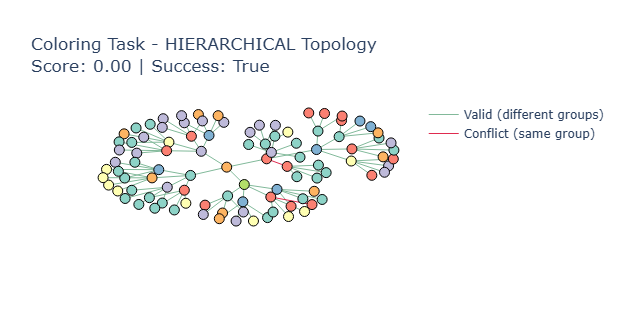
\includegraphics[trim=90 80 200 100,clip,width=0.26\textwidth]{figures/topology/coloring_results_20250925_000609_rounds15_gpt-4o-mini_nodes100}} \\

    \caption{Coloring experiment outcomes across different network sizes ($n=4$ to $100$). 
    Each subfigure shows the final group assignments of agents. 
    Valid assignments (neighbors in different groups) are shown in green, while conflicts (neighbors in the same group) are shown in red.}
    \label{fig:coloring-results}
\end{figure*}
